\section{Multiresolution TSDB model definition}

In this section we design a mathematical model for the multiresolution time series database management systems (MTSDB). Some concepts come from an abstraction of RRDtool operations \parencite{rrdtool}. 

A MTSDB manages time series. A time series is regarded as a chronological data collection, so it needs an appropriate management by the DBMS.
The MTSDB model is an storage solution for a time series where, in short,  the time series information is spread in different time resolutions. 

The main objects of a MTSDB are \emph{measures} and \emph{time series}. A \emph{measure} is a value measured in an instant in time and a  \emph{time series} is a collection of \emph{measures}. A database from a MTSDB contains one time series, which internally is stored in multiple resolutions of itself.

\begin{figure}[tp]
\centering
\setlength{\unitlength}{0.4mm}
% Graphic for TeX using PGF
% Title: /home/aleix/pfc_svn/imatges/model/arxiurrd.dia
% Creator: Dia v0.97.1
% CreationDate: Tue May 31 13:01:29 2011
% For: aleix
% \usepackage{tikz}
% The following commands are not supported in PSTricks at present
% We define them conditionally, so when they are implemented,
% this pgf file will use them.
\ifx\du\undefined
  \newlength{\du}
\fi
\setlength{\du}{15\unitlength}
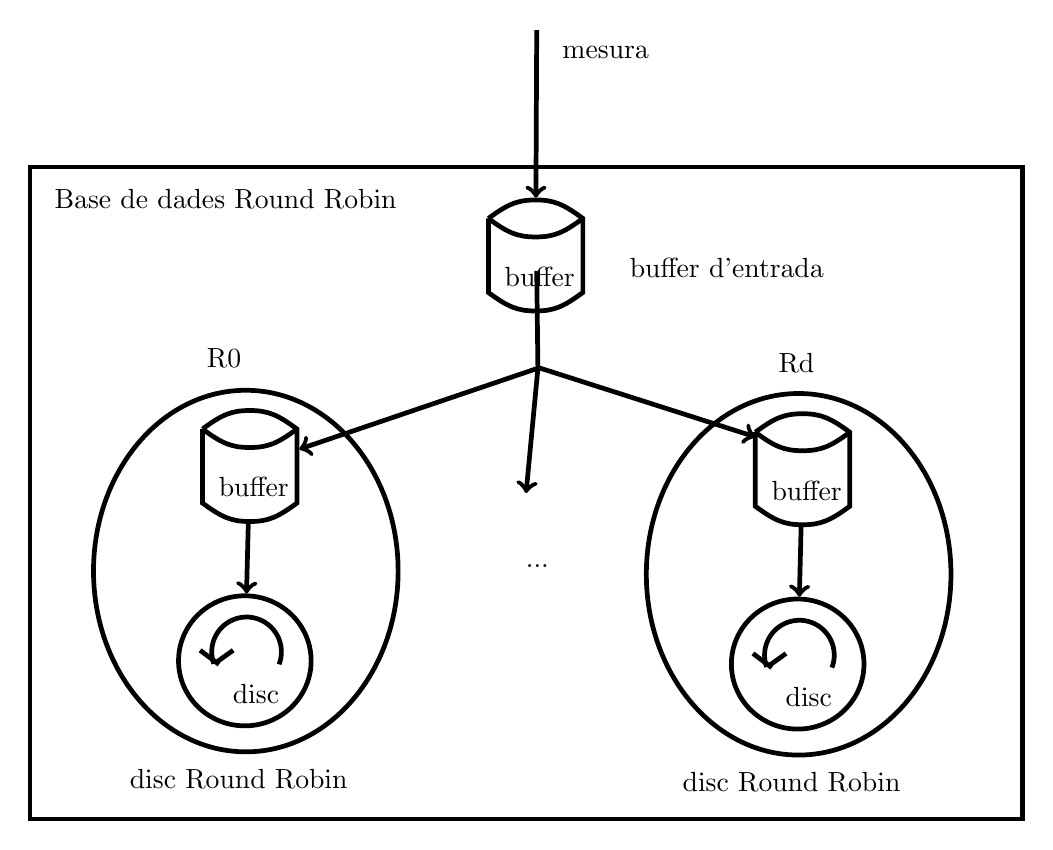
\begin{tikzpicture}
\pgftransformxscale{1.000000}
\pgftransformyscale{-1.000000}
\definecolor{dialinecolor}{rgb}{0.000000, 0.000000, 0.000000}
\pgfsetstrokecolor{dialinecolor}
\definecolor{dialinecolor}{rgb}{1.000000, 1.000000, 1.000000}
\pgfsetfillcolor{dialinecolor}
\definecolor{dialinecolor}{rgb}{1.000000, 1.000000, 1.000000}
\pgfsetfillcolor{dialinecolor}
\fill (7.200000\du,-9.403364\du)--(7.200000\du,4.396636\du)--(28.200000\du,4.396636\du)--(28.200000\du,-9.403364\du)--cycle;
\pgfsetlinewidth{0.100000\du}
\pgfsetdash{}{0pt}
\pgfsetdash{}{0pt}
\pgfsetmiterjoin
\definecolor{dialinecolor}{rgb}{0.000000, 0.000000, 0.000000}
\pgfsetstrokecolor{dialinecolor}
\draw (7.200000\du,-9.403364\du)--(7.200000\du,4.396636\du)--(28.200000\du,4.396636\du)--(28.200000\du,-9.403364\du)--cycle;
% setfont left to latex
\definecolor{dialinecolor}{rgb}{0.000000, 0.000000, 0.000000}
\pgfsetstrokecolor{dialinecolor}
\node at (17.700000\du,-2.308364\du){};
\definecolor{dialinecolor}{rgb}{1.000000, 1.000000, 1.000000}
\pgfsetfillcolor{dialinecolor}
\pgfpathellipse{\pgfpoint{11.767338\du}{-0.851682\du}}{\pgfpoint{3.224066\du}{0\du}}{\pgfpoint{0\du}{3.826682\du}}
\pgfusepath{fill}
\pgfsetlinewidth{0.100000\du}
\pgfsetdash{}{0pt}
\pgfsetdash{}{0pt}
\pgfsetmiterjoin
\definecolor{dialinecolor}{rgb}{0.000000, 0.000000, 0.000000}
\pgfsetstrokecolor{dialinecolor}
\pgfpathellipse{\pgfpoint{11.767338\du}{-0.851682\du}}{\pgfpoint{3.224066\du}{0\du}}{\pgfpoint{0\du}{3.826682\du}}
\pgfusepath{stroke}
% setfont left to latex
\definecolor{dialinecolor}{rgb}{0.000000, 0.000000, 0.000000}
\pgfsetstrokecolor{dialinecolor}
\node at (11.767338\du,-0.656682\du){};
\definecolor{dialinecolor}{rgb}{1.000000, 1.000000, 1.000000}
\pgfsetfillcolor{dialinecolor}
\pgfpathellipse{\pgfpoint{11.746636\du}{1.048318\du}}{\pgfpoint{1.403364\du}{0\du}}{\pgfpoint{0\du}{1.376682\du}}
\pgfusepath{fill}
\pgfsetlinewidth{0.100000\du}
\pgfsetdash{}{0pt}
\pgfsetdash{}{0pt}
\pgfsetmiterjoin
\definecolor{dialinecolor}{rgb}{0.000000, 0.000000, 0.000000}
\pgfsetstrokecolor{dialinecolor}
\pgfpathellipse{\pgfpoint{11.746636\du}{1.048318\du}}{\pgfpoint{1.403364\du}{0\du}}{\pgfpoint{0\du}{1.376682\du}}
\pgfusepath{stroke}
% setfont left to latex
\definecolor{dialinecolor}{rgb}{0.000000, 0.000000, 0.000000}
\pgfsetstrokecolor{dialinecolor}
\node at (11.746636\du,1.243318\du){};
\pgfsetlinewidth{0.100000\du}
\pgfsetdash{}{0pt}
\pgfsetdash{}{0pt}
\pgfsetbuttcap
\pgfsetmiterjoin
\pgfsetlinewidth{0.100000\du}
\pgfsetbuttcap
\pgfsetmiterjoin
\pgfsetdash{}{0pt}
\definecolor{dialinecolor}{rgb}{1.000000, 1.000000, 1.000000}
\pgfsetfillcolor{dialinecolor}
\pgfpathmoveto{\pgfpoint{10.850000\du}{-3.858333\du}}
\pgfpathcurveto{\pgfpoint{11.250000\du}{-4.152083\du}}{\pgfpoint{11.450000\du}{-4.250000\du}}{\pgfpoint{11.850000\du}{-4.250000\du}}
\pgfpathcurveto{\pgfpoint{12.250000\du}{-4.250000\du}}{\pgfpoint{12.450000\du}{-4.152083\du}}{\pgfpoint{12.850000\du}{-3.858333\du}}
\pgfpathlineto{\pgfpoint{12.850000\du}{-2.291667\du}}
\pgfpathcurveto{\pgfpoint{12.450000\du}{-1.997917\du}}{\pgfpoint{12.250000\du}{-1.900000\du}}{\pgfpoint{11.850000\du}{-1.900000\du}}
\pgfpathcurveto{\pgfpoint{11.450000\du}{-1.900000\du}}{\pgfpoint{11.250000\du}{-1.997917\du}}{\pgfpoint{10.850000\du}{-2.291667\du}}
\pgfpathlineto{\pgfpoint{10.850000\du}{-3.858333\du}}
\pgfusepath{fill}
\definecolor{dialinecolor}{rgb}{0.000000, 0.000000, 0.000000}
\pgfsetstrokecolor{dialinecolor}
\pgfpathmoveto{\pgfpoint{10.850000\du}{-3.858333\du}}
\pgfpathcurveto{\pgfpoint{11.250000\du}{-4.152083\du}}{\pgfpoint{11.450000\du}{-4.250000\du}}{\pgfpoint{11.850000\du}{-4.250000\du}}
\pgfpathcurveto{\pgfpoint{12.250000\du}{-4.250000\du}}{\pgfpoint{12.450000\du}{-4.152083\du}}{\pgfpoint{12.850000\du}{-3.858333\du}}
\pgfpathlineto{\pgfpoint{12.850000\du}{-2.291667\du}}
\pgfpathcurveto{\pgfpoint{12.450000\du}{-1.997917\du}}{\pgfpoint{12.250000\du}{-1.900000\du}}{\pgfpoint{11.850000\du}{-1.900000\du}}
\pgfpathcurveto{\pgfpoint{11.450000\du}{-1.900000\du}}{\pgfpoint{11.250000\du}{-1.997917\du}}{\pgfpoint{10.850000\du}{-2.291667\du}}
\pgfpathlineto{\pgfpoint{10.850000\du}{-3.858333\du}}
\pgfusepath{stroke}
\pgfsetbuttcap
\pgfsetmiterjoin
\pgfsetdash{}{0pt}
\definecolor{dialinecolor}{rgb}{0.000000, 0.000000, 0.000000}
\pgfsetstrokecolor{dialinecolor}
\pgfpathmoveto{\pgfpoint{10.850000\du}{-3.858333\du}}
\pgfpathcurveto{\pgfpoint{11.250000\du}{-3.564583\du}}{\pgfpoint{11.450000\du}{-3.466667\du}}{\pgfpoint{11.850000\du}{-3.466667\du}}
\pgfpathcurveto{\pgfpoint{12.250000\du}{-3.466667\du}}{\pgfpoint{12.450000\du}{-3.564583\du}}{\pgfpoint{12.850000\du}{-3.858333\du}}
\pgfusepath{stroke}
% setfont left to latex
\definecolor{dialinecolor}{rgb}{0.000000, 0.000000, 0.000000}
\pgfsetstrokecolor{dialinecolor}
\node at (11.850000\du,-2.679167\du){};
\pgfsetlinewidth{0.100000\du}
\pgfsetdash{}{0pt}
\pgfsetdash{}{0pt}
\pgfsetbuttcap
{
\definecolor{dialinecolor}{rgb}{0.000000, 0.000000, 0.000000}
\pgfsetfillcolor{dialinecolor}
% was here!!!
\definecolor{dialinecolor}{rgb}{0.000000, 0.000000, 0.000000}
\pgfsetstrokecolor{dialinecolor}
\pgfpathmoveto{\pgfpoint{12.471610\du}{1.123386\du}}
\pgfpatharc{21}{-200}{0.737486\du and 0.737486\du}
\pgfusepath{stroke}
}
\pgfsetlinewidth{0.100000\du}
\pgfsetdash{}{0pt}
\pgfsetdash{}{0pt}
\pgfsetbuttcap
{
\definecolor{dialinecolor}{rgb}{0.000000, 0.000000, 0.000000}
\pgfsetfillcolor{dialinecolor}
% was here!!!
\definecolor{dialinecolor}{rgb}{0.000000, 0.000000, 0.000000}
\pgfsetstrokecolor{dialinecolor}
\draw (16.171636\du,0.473318\du)--(16.171636\du,0.473318\du);
}
\pgfsetlinewidth{0.100000\du}
\pgfsetdash{}{0pt}
\pgfsetdash{}{0pt}
\pgfsetbuttcap
{
\definecolor{dialinecolor}{rgb}{0.000000, 0.000000, 0.000000}
\pgfsetfillcolor{dialinecolor}
% was here!!!
\definecolor{dialinecolor}{rgb}{0.000000, 0.000000, 0.000000}
\pgfsetstrokecolor{dialinecolor}
\draw (11.200000\du,1.125000\du)--(10.800000\du,0.825000\du);
}
\pgfsetlinewidth{0.100000\du}
\pgfsetdash{}{0pt}
\pgfsetdash{}{0pt}
\pgfsetbuttcap
{
\definecolor{dialinecolor}{rgb}{0.000000, 0.000000, 0.000000}
\pgfsetfillcolor{dialinecolor}
% was here!!!
\definecolor{dialinecolor}{rgb}{0.000000, 0.000000, 0.000000}
\pgfsetstrokecolor{dialinecolor}
\draw (11.150000\du,1.075000\du)--(11.500000\du,0.825000\du);
}
\pgfsetlinewidth{0.100000\du}
\pgfsetdash{}{0pt}
\pgfsetdash{}{0pt}
\pgfsetbuttcap
{
\definecolor{dialinecolor}{rgb}{0.000000, 0.000000, 0.000000}
\pgfsetfillcolor{dialinecolor}
% was here!!!
\pgfsetarrowsend{to}
\definecolor{dialinecolor}{rgb}{0.000000, 0.000000, 0.000000}
\pgfsetstrokecolor{dialinecolor}
\draw (11.819301\du,-1.850387\du)--(11.782382\du,-0.377629\du);
}
% setfont left to latex
\definecolor{dialinecolor}{rgb}{0.000000, 0.000000, 0.000000}
\pgfsetstrokecolor{dialinecolor}
\node[anchor=west] at (10.950000\du,-2.625000\du){buffer};
% setfont left to latex
\definecolor{dialinecolor}{rgb}{0.000000, 0.000000, 0.000000}
\pgfsetstrokecolor{dialinecolor}
\node[anchor=west] at (11.246636\du,1.748318\du){disc};
% setfont left to latex
\definecolor{dialinecolor}{rgb}{0.000000, 0.000000, 0.000000}
\pgfsetstrokecolor{dialinecolor}
\node[anchor=west] at (9.067338\du,3.548318\du){disc Round Robin};
\definecolor{dialinecolor}{rgb}{1.000000, 1.000000, 1.000000}
\pgfsetfillcolor{dialinecolor}
\pgfpathellipse{\pgfpoint{23.469066\du}{-0.783318\du}}{\pgfpoint{3.224066\du}{0\du}}{\pgfpoint{0\du}{3.826682\du}}
\pgfusepath{fill}
\pgfsetlinewidth{0.100000\du}
\pgfsetdash{}{0pt}
\pgfsetdash{}{0pt}
\pgfsetmiterjoin
\definecolor{dialinecolor}{rgb}{0.000000, 0.000000, 0.000000}
\pgfsetstrokecolor{dialinecolor}
\pgfpathellipse{\pgfpoint{23.469066\du}{-0.783318\du}}{\pgfpoint{3.224066\du}{0\du}}{\pgfpoint{0\du}{3.826682\du}}
\pgfusepath{stroke}
% setfont left to latex
\definecolor{dialinecolor}{rgb}{0.000000, 0.000000, 0.000000}
\pgfsetstrokecolor{dialinecolor}
\node at (23.469066\du,-0.588318\du){};
\definecolor{dialinecolor}{rgb}{1.000000, 1.000000, 1.000000}
\pgfsetfillcolor{dialinecolor}
\pgfpathellipse{\pgfpoint{23.448364\du}{1.116682\du}}{\pgfpoint{1.403364\du}{0\du}}{\pgfpoint{0\du}{1.376682\du}}
\pgfusepath{fill}
\pgfsetlinewidth{0.100000\du}
\pgfsetdash{}{0pt}
\pgfsetdash{}{0pt}
\pgfsetmiterjoin
\definecolor{dialinecolor}{rgb}{0.000000, 0.000000, 0.000000}
\pgfsetstrokecolor{dialinecolor}
\pgfpathellipse{\pgfpoint{23.448364\du}{1.116682\du}}{\pgfpoint{1.403364\du}{0\du}}{\pgfpoint{0\du}{1.376682\du}}
\pgfusepath{stroke}
% setfont left to latex
\definecolor{dialinecolor}{rgb}{0.000000, 0.000000, 0.000000}
\pgfsetstrokecolor{dialinecolor}
\node at (23.448364\du,1.311682\du){};
\pgfsetlinewidth{0.100000\du}
\pgfsetdash{}{0pt}
\pgfsetdash{}{0pt}
\pgfsetbuttcap
\pgfsetmiterjoin
\pgfsetlinewidth{0.100000\du}
\pgfsetbuttcap
\pgfsetmiterjoin
\pgfsetdash{}{0pt}
\definecolor{dialinecolor}{rgb}{1.000000, 1.000000, 1.000000}
\pgfsetfillcolor{dialinecolor}
\pgfpathmoveto{\pgfpoint{22.551728\du}{-3.789969\du}}
\pgfpathcurveto{\pgfpoint{22.951728\du}{-4.083719\du}}{\pgfpoint{23.151728\du}{-4.181636\du}}{\pgfpoint{23.551728\du}{-4.181636\du}}
\pgfpathcurveto{\pgfpoint{23.951728\du}{-4.181636\du}}{\pgfpoint{24.151728\du}{-4.083719\du}}{\pgfpoint{24.551728\du}{-3.789969\du}}
\pgfpathlineto{\pgfpoint{24.551728\du}{-2.223303\du}}
\pgfpathcurveto{\pgfpoint{24.151728\du}{-1.929553\du}}{\pgfpoint{23.951728\du}{-1.831636\du}}{\pgfpoint{23.551728\du}{-1.831636\du}}
\pgfpathcurveto{\pgfpoint{23.151728\du}{-1.831636\du}}{\pgfpoint{22.951728\du}{-1.929553\du}}{\pgfpoint{22.551728\du}{-2.223303\du}}
\pgfpathlineto{\pgfpoint{22.551728\du}{-3.789969\du}}
\pgfusepath{fill}
\definecolor{dialinecolor}{rgb}{0.000000, 0.000000, 0.000000}
\pgfsetstrokecolor{dialinecolor}
\pgfpathmoveto{\pgfpoint{22.551728\du}{-3.789969\du}}
\pgfpathcurveto{\pgfpoint{22.951728\du}{-4.083719\du}}{\pgfpoint{23.151728\du}{-4.181636\du}}{\pgfpoint{23.551728\du}{-4.181636\du}}
\pgfpathcurveto{\pgfpoint{23.951728\du}{-4.181636\du}}{\pgfpoint{24.151728\du}{-4.083719\du}}{\pgfpoint{24.551728\du}{-3.789969\du}}
\pgfpathlineto{\pgfpoint{24.551728\du}{-2.223303\du}}
\pgfpathcurveto{\pgfpoint{24.151728\du}{-1.929553\du}}{\pgfpoint{23.951728\du}{-1.831636\du}}{\pgfpoint{23.551728\du}{-1.831636\du}}
\pgfpathcurveto{\pgfpoint{23.151728\du}{-1.831636\du}}{\pgfpoint{22.951728\du}{-1.929553\du}}{\pgfpoint{22.551728\du}{-2.223303\du}}
\pgfpathlineto{\pgfpoint{22.551728\du}{-3.789969\du}}
\pgfusepath{stroke}
\pgfsetbuttcap
\pgfsetmiterjoin
\pgfsetdash{}{0pt}
\definecolor{dialinecolor}{rgb}{0.000000, 0.000000, 0.000000}
\pgfsetstrokecolor{dialinecolor}
\pgfpathmoveto{\pgfpoint{22.551728\du}{-3.789969\du}}
\pgfpathcurveto{\pgfpoint{22.951728\du}{-3.496219\du}}{\pgfpoint{23.151728\du}{-3.398303\du}}{\pgfpoint{23.551728\du}{-3.398303\du}}
\pgfpathcurveto{\pgfpoint{23.951728\du}{-3.398303\du}}{\pgfpoint{24.151728\du}{-3.496219\du}}{\pgfpoint{24.551728\du}{-3.789969\du}}
\pgfusepath{stroke}
% setfont left to latex
\definecolor{dialinecolor}{rgb}{0.000000, 0.000000, 0.000000}
\pgfsetstrokecolor{dialinecolor}
\node at (23.551728\du,-2.610803\du){};
\pgfsetlinewidth{0.100000\du}
\pgfsetdash{}{0pt}
\pgfsetdash{}{0pt}
\pgfsetbuttcap
{
\definecolor{dialinecolor}{rgb}{0.000000, 0.000000, 0.000000}
\pgfsetfillcolor{dialinecolor}
% was here!!!
\definecolor{dialinecolor}{rgb}{0.000000, 0.000000, 0.000000}
\pgfsetstrokecolor{dialinecolor}
\pgfpathmoveto{\pgfpoint{24.173338\du}{1.191750\du}}
\pgfpatharc{21}{-200}{0.737486\du and 0.737486\du}
\pgfusepath{stroke}
}
\pgfsetlinewidth{0.100000\du}
\pgfsetdash{}{0pt}
\pgfsetdash{}{0pt}
\pgfsetbuttcap
{
\definecolor{dialinecolor}{rgb}{0.000000, 0.000000, 0.000000}
\pgfsetfillcolor{dialinecolor}
% was here!!!
\definecolor{dialinecolor}{rgb}{0.000000, 0.000000, 0.000000}
\pgfsetstrokecolor{dialinecolor}
\draw (27.873364\du,0.541682\du)--(27.873364\du,0.541682\du);
}
\pgfsetlinewidth{0.100000\du}
\pgfsetdash{}{0pt}
\pgfsetdash{}{0pt}
\pgfsetbuttcap
{
\definecolor{dialinecolor}{rgb}{0.000000, 0.000000, 0.000000}
\pgfsetfillcolor{dialinecolor}
% was here!!!
\definecolor{dialinecolor}{rgb}{0.000000, 0.000000, 0.000000}
\pgfsetstrokecolor{dialinecolor}
\draw (22.901728\du,1.193364\du)--(22.501728\du,0.893364\du);
}
\pgfsetlinewidth{0.100000\du}
\pgfsetdash{}{0pt}
\pgfsetdash{}{0pt}
\pgfsetbuttcap
{
\definecolor{dialinecolor}{rgb}{0.000000, 0.000000, 0.000000}
\pgfsetfillcolor{dialinecolor}
% was here!!!
\definecolor{dialinecolor}{rgb}{0.000000, 0.000000, 0.000000}
\pgfsetstrokecolor{dialinecolor}
\draw (22.851728\du,1.143364\du)--(23.201728\du,0.893364\du);
}
\pgfsetlinewidth{0.100000\du}
\pgfsetdash{}{0pt}
\pgfsetdash{}{0pt}
\pgfsetbuttcap
{
\definecolor{dialinecolor}{rgb}{0.000000, 0.000000, 0.000000}
\pgfsetfillcolor{dialinecolor}
% was here!!!
\pgfsetarrowsend{to}
\definecolor{dialinecolor}{rgb}{0.000000, 0.000000, 0.000000}
\pgfsetstrokecolor{dialinecolor}
\draw (23.521029\du,-1.782023\du)--(23.484110\du,-0.309265\du);
}
% setfont left to latex
\definecolor{dialinecolor}{rgb}{0.000000, 0.000000, 0.000000}
\pgfsetstrokecolor{dialinecolor}
\node[anchor=west] at (22.651728\du,-2.556636\du){buffer};
% setfont left to latex
\definecolor{dialinecolor}{rgb}{0.000000, 0.000000, 0.000000}
\pgfsetstrokecolor{dialinecolor}
\node[anchor=west] at (22.948364\du,1.816682\du){disc};
% setfont left to latex
\definecolor{dialinecolor}{rgb}{0.000000, 0.000000, 0.000000}
\pgfsetstrokecolor{dialinecolor}
\node[anchor=west] at (20.769066\du,3.616682\du){disc Round Robin};
% setfont left to latex
\definecolor{dialinecolor}{rgb}{0.000000, 0.000000, 0.000000}
\pgfsetstrokecolor{dialinecolor}
\node[anchor=west] at (17.450000\du,-0.950000\du){...};
% setfont left to latex
\definecolor{dialinecolor}{rgb}{0.000000, 0.000000, 0.000000}
\pgfsetstrokecolor{dialinecolor}
\node[anchor=west] at (10.700000\du,-5.350000\du){R0};
% setfont left to latex
\definecolor{dialinecolor}{rgb}{0.000000, 0.000000, 0.000000}
\pgfsetstrokecolor{dialinecolor}
\node[anchor=west] at (22.800000\du,-5.250000\du){Rd};
\pgfsetlinewidth{0.100000\du}
\pgfsetdash{}{0pt}
\pgfsetdash{}{0pt}
\pgfsetbuttcap
{
\definecolor{dialinecolor}{rgb}{0.000000, 0.000000, 0.000000}
\pgfsetfillcolor{dialinecolor}
% was here!!!
\definecolor{dialinecolor}{rgb}{0.000000, 0.000000, 0.000000}
\pgfsetstrokecolor{dialinecolor}
\draw (10.123364\du,-7.233318\du)--(10.123364\du,-7.233318\du);
}
\pgfsetlinewidth{0.100000\du}
\pgfsetdash{}{0pt}
\pgfsetdash{}{0pt}
\pgfsetbuttcap
\pgfsetmiterjoin
\pgfsetlinewidth{0.100000\du}
\pgfsetbuttcap
\pgfsetmiterjoin
\pgfsetdash{}{0pt}
\definecolor{dialinecolor}{rgb}{1.000000, 1.000000, 1.000000}
\pgfsetfillcolor{dialinecolor}
\pgfpathmoveto{\pgfpoint{16.901728\du}{-8.314969\du}}
\pgfpathcurveto{\pgfpoint{17.301728\du}{-8.608719\du}}{\pgfpoint{17.501728\du}{-8.706636\du}}{\pgfpoint{17.901728\du}{-8.706636\du}}
\pgfpathcurveto{\pgfpoint{18.301728\du}{-8.706636\du}}{\pgfpoint{18.501728\du}{-8.608719\du}}{\pgfpoint{18.901728\du}{-8.314969\du}}
\pgfpathlineto{\pgfpoint{18.901728\du}{-6.748303\du}}
\pgfpathcurveto{\pgfpoint{18.501728\du}{-6.454553\du}}{\pgfpoint{18.301728\du}{-6.356636\du}}{\pgfpoint{17.901728\du}{-6.356636\du}}
\pgfpathcurveto{\pgfpoint{17.501728\du}{-6.356636\du}}{\pgfpoint{17.301728\du}{-6.454553\du}}{\pgfpoint{16.901728\du}{-6.748303\du}}
\pgfpathlineto{\pgfpoint{16.901728\du}{-8.314969\du}}
\pgfusepath{fill}
\definecolor{dialinecolor}{rgb}{0.000000, 0.000000, 0.000000}
\pgfsetstrokecolor{dialinecolor}
\pgfpathmoveto{\pgfpoint{16.901728\du}{-8.314969\du}}
\pgfpathcurveto{\pgfpoint{17.301728\du}{-8.608719\du}}{\pgfpoint{17.501728\du}{-8.706636\du}}{\pgfpoint{17.901728\du}{-8.706636\du}}
\pgfpathcurveto{\pgfpoint{18.301728\du}{-8.706636\du}}{\pgfpoint{18.501728\du}{-8.608719\du}}{\pgfpoint{18.901728\du}{-8.314969\du}}
\pgfpathlineto{\pgfpoint{18.901728\du}{-6.748303\du}}
\pgfpathcurveto{\pgfpoint{18.501728\du}{-6.454553\du}}{\pgfpoint{18.301728\du}{-6.356636\du}}{\pgfpoint{17.901728\du}{-6.356636\du}}
\pgfpathcurveto{\pgfpoint{17.501728\du}{-6.356636\du}}{\pgfpoint{17.301728\du}{-6.454553\du}}{\pgfpoint{16.901728\du}{-6.748303\du}}
\pgfpathlineto{\pgfpoint{16.901728\du}{-8.314969\du}}
\pgfusepath{stroke}
\pgfsetbuttcap
\pgfsetmiterjoin
\pgfsetdash{}{0pt}
\definecolor{dialinecolor}{rgb}{0.000000, 0.000000, 0.000000}
\pgfsetstrokecolor{dialinecolor}
\pgfpathmoveto{\pgfpoint{16.901728\du}{-8.314969\du}}
\pgfpathcurveto{\pgfpoint{17.301728\du}{-8.021219\du}}{\pgfpoint{17.501728\du}{-7.923303\du}}{\pgfpoint{17.901728\du}{-7.923303\du}}
\pgfpathcurveto{\pgfpoint{18.301728\du}{-7.923303\du}}{\pgfpoint{18.501728\du}{-8.021219\du}}{\pgfpoint{18.901728\du}{-8.314969\du}}
\pgfusepath{stroke}
% setfont left to latex
\definecolor{dialinecolor}{rgb}{0.000000, 0.000000, 0.000000}
\pgfsetstrokecolor{dialinecolor}
\node at (17.901728\du,-7.135803\du){};
% setfont left to latex
\definecolor{dialinecolor}{rgb}{0.000000, 0.000000, 0.000000}
\pgfsetstrokecolor{dialinecolor}
\node[anchor=west] at (17.001728\du,-7.081636\du){buffer};
% setfont left to latex
\definecolor{dialinecolor}{rgb}{0.000000, 0.000000, 0.000000}
\pgfsetstrokecolor{dialinecolor}
\node[anchor=west] at (19.650000\du,-7.278364\du){buffer d'entrada};
\pgfsetlinewidth{0.100000\du}
\pgfsetdash{}{0pt}
\pgfsetdash{}{0pt}
\pgfsetbuttcap
{
\definecolor{dialinecolor}{rgb}{0.000000, 0.000000, 0.000000}
\pgfsetfillcolor{dialinecolor}
% was here!!!
\pgfsetarrowsend{to}
\definecolor{dialinecolor}{rgb}{0.000000, 0.000000, 0.000000}
\pgfsetstrokecolor{dialinecolor}
\draw (17.975000\du,-5.153364\du)--(12.900117\du,-3.431331\du);
}
\pgfsetlinewidth{0.100000\du}
\pgfsetdash{}{0pt}
\pgfsetdash{}{0pt}
\pgfsetbuttcap
{
\definecolor{dialinecolor}{rgb}{0.000000, 0.000000, 0.000000}
\pgfsetfillcolor{dialinecolor}
% was here!!!
\definecolor{dialinecolor}{rgb}{0.000000, 0.000000, 0.000000}
\pgfsetstrokecolor{dialinecolor}
\draw (17.925000\du,-7.203364\du)--(17.950000\du,-5.128364\du);
}
\pgfsetlinewidth{0.100000\du}
\pgfsetdash{}{0pt}
\pgfsetdash{}{0pt}
\pgfsetbuttcap
{
\definecolor{dialinecolor}{rgb}{0.000000, 0.000000, 0.000000}
\pgfsetfillcolor{dialinecolor}
% was here!!!
\pgfsetarrowsend{to}
\definecolor{dialinecolor}{rgb}{0.000000, 0.000000, 0.000000}
\pgfsetstrokecolor{dialinecolor}
\draw (17.950000\du,-5.140864\du)--(17.700000\du,-2.503364\du);
}
\pgfsetlinewidth{0.100000\du}
\pgfsetdash{}{0pt}
\pgfsetdash{}{0pt}
\pgfsetbuttcap
{
\definecolor{dialinecolor}{rgb}{0.000000, 0.000000, 0.000000}
\pgfsetfillcolor{dialinecolor}
% was here!!!
\pgfsetarrowsstart{to}
\definecolor{dialinecolor}{rgb}{0.000000, 0.000000, 0.000000}
\pgfsetstrokecolor{dialinecolor}
\draw (22.551728\du,-3.692053\du)--(17.975000\du,-5.153364\du);
}
\pgfsetlinewidth{0.100000\du}
\pgfsetdash{}{0pt}
\pgfsetdash{}{0pt}
\pgfsetbuttcap
{
\definecolor{dialinecolor}{rgb}{0.000000, 0.000000, 0.000000}
\pgfsetfillcolor{dialinecolor}
% was here!!!
\pgfsetarrowsend{to}
\definecolor{dialinecolor}{rgb}{0.000000, 0.000000, 0.000000}
\pgfsetstrokecolor{dialinecolor}
\draw (17.925000\du,-12.303364\du)--(17.907694\du,-8.754857\du);
}
% setfont left to latex
\definecolor{dialinecolor}{rgb}{0.000000, 0.000000, 0.000000}
\pgfsetstrokecolor{dialinecolor}
\node[anchor=west] at (18.225000\du,-11.828364\du){mesura};
% setfont left to latex
\definecolor{dialinecolor}{rgb}{0.000000, 0.000000, 0.000000}
\pgfsetstrokecolor{dialinecolor}
\node[anchor=west] at (7.475000\du,-8.728364\du){Base de dades Round Robin};
\end{tikzpicture}

\caption{Architecture of MTSDB model}
\label{fig:model:mtsdb}
\end{figure}

The general schema of the MTSDB model can be seen in figure \ref{fig:model:mtsdb}.  A \emph{multiresolution database} is a collection of \emph{resolution discs}, which temporarily accumulate the \emph{measures} in a \emph{buffer} where they are processed and finally stored in a \emph{disc}. Mainly, the data process is intended to change the time intervals between \emph{measures} in order to compact the time series information. In this way, the time series gets stored in different time resolutions, which are spread in the \emph{discs}.

\emph{Discs} are size bounded so they only contain a fixed amount of \emph{measures}. When a \emph{disc} gets full it discards a \emph{measure}. In this way, the multiresolution database is bounded in size and the time series gets stored in pieces, that is 'time subseries'.



\begin{figure}[tp]
\centering
\tiny
\setlength{\unitlength}{2mm}
\begin{center}
\begin{multicols}{3} 


    \begin{picture}(14,12)(-7,-6)
    \put(0,-1){\makebox(0,0)[c]{{\color{blue}5 dies}}}
      \put(0,0){\circle{10}}
      \put(5,0){\circle{0.8}}
      \put(2.5,4.33){\circle{0.8}}
      \put(-2.5,4.33){\circle{0.8}}   
      \put(-5,0){\circle{0.8}}
      \put(-2.5,-4.33){\circle{0.8}} 
      \put(2.5,-4.33){\circle{0.8}} 
      \put(0,0){\vector(0,1){5}}
      \put(0,0){\oval(5,5)[t]}
      \put(-2.5,0){\makebox(0,0)[c]{$\vee$}}
    \end{picture}


    \begin{picture}(14,12)(-7,-6)
    \put(0,-1){\makebox(0,0)[c]{{\color{red}1 dia}}}
      \put(0,0){\circle{10}}
      \put(5,0){\circle{0.8}}
      \put(4.33,2.5){\circle{0.8}}
      \put(2.5,4.33){\circle{0.8}}
      \put(0,5){\circle{0.8}}
      \put(-2.5,4.33){\circle{0.8}}   
      \put(-4.33,2.5){\circle{0.8}}
      \put(-5,0){\circle{0.8}}
      \put(-4.33,-2.5){\circle{0.8}}
      \put(-2.5,-4.33){\circle{0.8}} 
      \put(0,-5){\circle{0.8}}
      \put(2.5,-4.33){\circle{0.8}} 
      \put(4.33,-2.5){\circle{0.8}}
      \put(0,0){\vector(0,1){5}}
      \put(0,0){\oval(5,5)[t]}
      \put(-2.5,0){\makebox(0,0)[c]{$\vee$}}
    \end{picture}

    \tiny
    \begin{picture}(14,12)(-7,-6)
    \put(0,-1){\makebox(0,0)[c]{{\color{green}5 min.}}}
      \put(0,0){\circle{10}}
      \put(5,0){\circle{0.8}}
      \put(4.82,1.29){\circle{0.8}}
      \put(4.33,2.5){\circle{0.8}}
     \put(3.5,3.5){\circle{0.8}}
      \put(2.5,4.33){\circle{0.8}}
      \put(1.29,4.82){\circle{0.8}}
      \put(0,5){\circle{0.8}}
      \put(-1.29,4.82){\circle{0.8}}
      \put(-2.5,4.33){\circle{0.8}}
       \put(-3.5,3.5){\circle{0.8}} 
      \put(-4.33,2.5){\circle{0.8}}
    \put(-4.82,1.29){\circle{0.8}}
      \put(-5,0){\circle{0.8}}
    \put(-4.82,-1.29){\circle{0.8}}
      \put(-4.33,-2.5){\circle{0.8}}
      \put(-3.5,-3.5){\circle{0.8}} 
      \put(-2.5,-4.33){\circle{0.8 } } 
      \put(-1.29,-4.82){}
\put(0,-5){\makebox(0,0)[c]{{[\dots\!]}}}
     \put(1.29,-4.82){}
      \put(2.5,-4.33){\circle{0.8}}
      \put(3.5,-3.5){\circle{0.8}} 
      \put(4.33,-2.5){\circle{0.8}}
  \put(4.82,-1.29){\circle{0.8}}
      \put(0,0){\vector(0,1){5}}
      \put(0,0){\oval(5,5)[t]}
      \put(-2.5,0){\makebox(0,0)[c]{$\vee$}}
    \end{picture}


\end{multicols}

\vspace{-10pt}

\setlength{\unitlength}{900sp}
\begin{picture}(14460,5066)(7322,-7927)
\thinlines
{\color[rgb]{0,0,0}\put(7300,-6271){\line( 0,-1){386}}
}%
{\color[rgb]{0,0,0}\put(7782,-6271){\line( 0,-1){386}}
}%
{\color[rgb]{0,0,0}\put(8263,-6271){\line( 0,-1){386}}
}%
{\color[rgb]{0,0,0}\put(8745,-6271){\line( 0,-1){386}}
}%
{\color[rgb]{0,0,0}\put(9227,-6271){\line( 0,-1){386}}
}%
{\color[rgb]{0,0,0}\put(9709,-6271){\line( 0,-1){386}}
}%
{\color[rgb]{0,0,0}\put(10191,-6271){\line( 0,-1){386}}
}%
{\color[rgb]{0,0,0}\put(10673,-6271){\line( 0,-1){386}}
}%
{\color[rgb]{0,0,0}\put(11155,-6271){\line( 0,-1){386}}
}%
{\color[rgb]{0,0,0}\put(11637,-6271){\line( 0,-1){386}}
}%
{\color[rgb]{0,0,0}\put(12119,-6271){\line( 0,-1){386}}
}%
{\color[rgb]{0,0,0}\put(12600,-6271){\line( 0,-1){386}}
}%
{\color[rgb]{0,0,0}\put(13082,-6271){\line( 0,-1){386}}
}%
{\color[rgb]{0,0,0}\put(13564,-6271){\line( 0,-1){386}}
}%
{\color[rgb]{0,0,0}\put(14046,-6271){\line( 0,-1){386}}
}%
{\color[rgb]{0,0,0}\put(14528,-6271){\line( 0,-1){386}}
}%
{\color[rgb]{0,0,0}\put(15010,-6271){\line( 0,-1){386}}
}%
{\color[rgb]{0,0,0}\put(15492,-6271){\line( 0,-1){386}}
}%
{\color[rgb]{0,0,0}\put(15974,-6271){\line( 0,-1){386}}
}%
{\color[rgb]{0,0,0}\put(16456,-6271){\line( 0,-1){386}}
}%
{\color[rgb]{0,0,0}\put(16938,-6271){\line( 0,-1){386}}
}%
{\color[rgb]{0,0,0}\put(17419,-6271){\line( 0,-1){386}}
}%
{\color[rgb]{0,0,0}\put(17901,-6271){\line( 0,-1){386}}
}%
{\color[rgb]{0,0,0}\put(18383,-6271){\line( 0,-1){386}}
}%
{\color[rgb]{0,0,0}\put(18865,-6271){\line( 0,-1){386}}
}%
{\color[rgb]{0,0,0}\put(19347,-6271){\line( 0,-1){386}}
}%
{\color[rgb]{0,0,0}\put(19829,-6271){\line( 0,-1){386}}
}%
{\color[rgb]{0,0,0}\put(20311,-6271){\line( 0,-1){386}}
}%
{\color[rgb]{0,0,0}\put(20793,-6271){\line( 0,-1){386}}
}%
{\color[rgb]{0,0,0}\put(21275,-6271){\line( 0,-1){386}}
}%
{\color[rgb]{0,0,0}\put(7300,-6271){\line( 0,-1){1157}}
}%
{\color[rgb]{0,0,0}\put(9709,-6271){\line( 0,-1){1157}}
}%
{\color[rgb]{0,0,0}\put(12119,-6271){\line( 0,-1){1157}}
}%
{\color[rgb]{0,0,0}\put(14528,-6271){\line( 0,-1){1157}}
}%
{\color[rgb]{0,0,0}\put(16938,-6271){\line( 0,-1){1157}}
}%
{\color[rgb]{0,0,0}\put(19347,-6271){\line( 0,-1){1157}}
}%
{\color[rgb]{0,0,0}\put(21756,-6271){\line( 0,-1){1157}}
}%
{\color[rgb]{0,0,0}\put(7300,-6271){\line( 1, 0){14456}}
}%

\put(7322,-6271){\line( 0,1){3000}}
\put(21756,-7783){\makebox(0,0)[b]{30 dies}}%

\color{blue}
\put(21782,-5928){\line( -1,0){14460}}
\put(21782,-5928){\line( 0,1){779}}
\put(21782,-5149){\line( -1,0){14460}}
\put(7322,-5928){\line( 0,1){779}}
\put(14530,-5450){\makebox(0,0)[c]{1 mes}}

\color{red}
\put(21782,-5149){\line( 0,1){779}}
\put(21782,-4370){\line( -1,0){5772}}
\put(16010,-5149){\line( 0,1){779}}
\put(18700,-4800){\makebox(0,0)[c]{12 dies}}

\color{green}
\put(21782,-4370){\line( 0,1){779}}
\put(21782,-3591){\line( -1,0){962}}
\put(20820,-4370){\line( 0,1){779}}
\put(21400,-3950){\makebox(0,0)[c]{2 d}}
\end{picture}%


\normalsize

\end{center}
\caption{Example of different resolutions for a time series in a MTSDB}
\label{fig:model:window}
\end{figure}

Putting resolution and 'time subseries' together, in a multiresolution database a time series is stored in different resolution pieces. For example, we could have a time series stored with high resolution at recent times and with low resolution at older times. This example is illustrated in figure \ref{fig:model:window}. At the top there are three \emph{discs} with different number of \emph{measures} and at the bottom there is a timeline showing the time series chopped along time. For recent times, every 5 minutes a \emph{measure} is stored in the third \emph{disc} which has a capacity of 576 \emph{measures} so that results in a 2 day piece. For mid times, every 1 day a  \emph{measure} is stored in the second \emph{disc} which has a capacity of 12 \emph{measures} so that results in a 12 days piece. For old times, every 5 days a  \emph{measure} is stored in the first \emph{disc} which has a capacity of 6 \emph{measures} so that results in a 30 days piece. 


Regarding operations, MTSDB model needs operators to change the time intervals between measures. Mainly, these operators are \emph{interpolation} functions and \emph{consolidation} actions. In this section we design the basic MTSDB model, that is six basic data model definitions -- \emph{measure}, \emph{time series}, \emph{buffer}, \emph{disc}, \emph{resolution disc}, and \emph{multiresolution database} -- and the operations to create a \emph{multiresolution database}, to add \emph{measures} and to \emph{interpolate} and \emph{consolidate} time series.



\subsection{Measure}

\begin{definition}[Measure]
  \label{def:measure}
  A \emph{measure} is a tuple $(v,t)$ where $v\in{\mathbb{R}}$ is the
  value of the measure and $t \in \mathbb{R}$ is the instant in time
  of measurement.
\end{definition}

Let $m=(v,t)$ be a measure, $v$ is written as $V(m)$ and $t$
is written as $T(m)$.

% \begin{definition}[Time]
%   \label{def:time}
%   Let $t^i_i$ and $t^i_j$ be two instants in time, we define the
%   amount of time or duration $t^d$ as the value $t^d \in\mathbb{R}$
%   measuring the distance in time units between the two instants $t^d =
%   t^i_i - t^i_j$.

%   Let $t^d$ be a duration and $t^{R}$ an instant in time of reference,
%   we define the instant in time $t^i$ as the value $t^i \in\mathbb{R}$
%   measuring the amount of time from the time of reference $t^i= t^{R}
%   + t^d$. The value of the time of reference is also an instant in
%   time but it can define exactly the position of any other instant in
%   time.

%   This definition is coherent with the one given in coordinate
%   systems, \cite{wiki:coordinate}.  Time is treated as universal and
%   constant. Time values are expressed in time units, that is seconds
%   in the international system.
% \end{definition}

The time value defines the order between measures.

\begin{definition}
  \label{def:order-relation}
  Let $m=(v_m,t_m)$ and $n=(v_n,t_n)$ be two measures, then $m\geq n$
  if and only if $t_m\geq t_n$.
\end{definition}

\subsection{Time series}

Time series are sequences of measures that are ordered in time. They
are also called time sequences such as in chapter two in \cite{last}.

\begin{definition}[Time series]
  A \emph{time series} $S$ is defined as a set of measures
  $S=\{m_0,\ldots,m_k\}$ without repeated time values $\forall i,j:
  i\leq k, j\leq k, i\neq j : T(m_i)\neq T(m_j)$. We will refer to the
  number of measures of the time series as the cardinality of the set
  $|S|$.
\end{definition}

The order defined in \ref{def:order-relation} implies a total order in
a time series. As a time series is a finite set, if it is not empty it
has a maximum and a minimum. 

\begin{definition}
  Let $S=\{m_0,\ldots,m_k\}$ be a time series and $n\in S$ be a
  measure. The time series' maximum is $n=\max(S)$ if and only if
  $\forall m \in S: n \geq m $.  Similarly, the time series' minimum
  is $n=\min(S)$ if and only if $\forall m \in S: n \leq m$.
\end{definition}

Given the order defined by time in a time series, we define the
sequence interval similarly as it is done in chapters 1 and 2 in \cite{last}.

\begin{definition}
  Let $S=\{m_0, \ldots, m_k\}$ be a time series. We define the subset
  $S(r,t] \subseteq S$ as the time series $S(r,t]=\{m\in S |
  r<T(m)\leq t\}$, where $r$ and $t$ are two instants in time.

  We also define the subset $S(r,+\infty)\subseteq S$ as the time
  series $S(r,+\infty) = \{m\in S | r< T(m) \leq T(\max(S))\}$ and the
  subset $S(-\infty,t)\subseteq S$ as the time series $S(-\infty,t) =
  \{m\in S | T(\min(S))\leq T(m) < t\}$.
\end{definition}

The time order in time series also implies the sequence concept of
next and previous measure.

\begin{definition}
  Let $S=\{m_0, \ldots, m_k\}$ be a time series and $l\in S$ and $n$
  two measures. We define the next measure of $n$ in $S$ as
  $\nex\limits_S(n) = \min(S(T(n),+\infty))$. We define the previous
  measure of $n$ in $S$ as $\prev\limits_S(n) =
  \max(S(-\infty,T(n)))$.
\end{definition}




\subsubsection{Regularity of time series} 

Let $S=\{m_0,\ldots,m_k\}$ be a time series, $t$ an instant in temps
and $\delta$ a duration of time, the time series' measures can be
situated in the time interval $i_0=[t,t+\delta]$ and its multiples
$i_j=[t+j\delta \,,\, t+(j+1)\delta]: j=0,1,2,\ldots$. When the
measures are equally spaced the time series is called regular.

\begin{definition}[Regular time series]
  Let $S=\{m_0,\ldots,m_k\}$ be a time series, $t$ an instant in time
  and $\delta$ a duration of time. We define $S$ as regular if and
  only if $\forall m \in S(T(\min(S),+\infty):T(m) - T(\prev(m)) =
  \delta$ and $T(\min(S))=t$.
\end{definition}

In signal processing, these time intervals are called sampling
intervals, $\delta$ is called sampling period and $t$ is called
sampling initial time.  


\subsection{Buffer}\label{sec:model:buffer}

A buffer is a container for a regular or a no-regular time series. The
buffer regularises the time series with a function to a constant
sampling period. We call consolidation to this action. In the context
of buffers, the constant sampling period is called consolidation step
and the function is called interpolation.

\begin{definition}[Buffer]
  A \emph{buffer} is defined as the tuple $(S,\tau,\delta,f)$ where
  $S$ is a time series, $\tau$ is the last consolidation instant in
  time, $\delta$ is the duration of the consolidation step and $f$ is
  an interpolation.
\end{definition}

An empty buffer, or the initial buffer, $B_{\emptyset} =
(\emptyset,t_0, \delta_0, f)$ is a buffer that has an empty time
series, the initial time of consolidation a duration indicating the
consolidation step and an interpolation. From the empty buffer all the
instants in time of consolidation can be calculated as $t_0+k\delta,
k\in\mathbb{N}$. Before the consolidation the buffer needs measures.

\begin{definition}
  The operator \emph{add} adds a measure to the time series of a buffer:
  \[
  \text{add}: \text{Buffer} \times \text{Measure} \longrightarrow \text{Buffer}
  \]
  \[
   B = (S,\tau,\delta,f)  \times m = (v,t) \mapsto B'= (S',\tau,\delta,f),
   S' = S \cup \{m\}
   \] 
\end{definition}

\begin{definition}
  We say the buffer is ready to consolidate when a time of a measure
  is bigger than the buffer's next instant in time of consolidation.
  Let $B=(S,\tau,\delta,f)$ be a buffer and $m=\max(S)$ the maximum
  measure, $B$ is ready to consolidate if and only if $T(m) \geq
  \tau+\delta$.
\end{definition}

Let $S$ be a time series and $t_0$ and $t_f$ two instants in time, an
interpolation function $f$ calculates a measure that is a summary of
$S$ in the time interval $i=[T_0,T_f]$:
\[
f: \text{Time series} \times \text{time interval} \longrightarrow
\text{Measure}
\]


In the design of the interpolation function we can interpret a time
series in different ways. Keogh at chapter 1 in \cite{last}, cites
some possible representations for time series such as \emph{Fourier
  Transforms}, \emph{Wavelets}, \emph{Symbolic Mappings} or
\emph{Piecewise Linear Representation} (PLR), remarking this last as
the most used. The most common representation is with linear
functions \parencite{keogh01}.

It is also possible to represent a time series with staircase
function, that is with a piecewise constant representation. In signal
theory it is widely used in digital-to-analog converter and the model
is known as \emph{zero-order hold}, which consists in holding each
value until the following value. Extending this model we define a new
interpretation for time series called \emph{zero-order hold backwards}
that is the representation used by RRDtool \parencite{lisa98:oetiker}.

\emph{Zero-order hold backwards} consists in holding each value until
the preceding value. Next, it is exemplified with a continuous
definition of a time series using left-continuous step functions.

\begin{definition}[zero-order hold backwards]
  Let $S=\{m_0,\ldots,m_k\}$ be a time series, $S(t)$ is the
  continuous representations along time $t$:
\[
\forall t \in \mathbb{R}  ,\forall m \in S:
S(t) =  
\begin{cases}
  \text{not defined} & \text{if } t > T(\max S) \\
  V(m) & \text{if }  t\in (T(\prev m),T(m)]
\end{cases}
\]
\end{definition}


There can be different interpolation functions in order to summarise a
time series. The representation of the time series can also make
differences to the same interpolation functions. Below are some
examples for time series represented by \emph{zero-order hold
  backwards}, where the time interval of consolidation is interpreted
left-continuous $(T_0,T_f]$.



\begin{definition}[Interpolation examples]
  Let $S=\{m_0,\ldots,m_k\}$ be a time series interpreted
  \emph{zero-order hold backwards} and $i=[T_0,T_f]$ be a time
  interval, the interpolation function summarises $S$ with a measure
  that is calculated from the measure values belonging to the subset
  $S(T_0,T_f]$:
  \[
  f: \text{Time series} \times \text{time interval}
  \longrightarrow \text{Measure}
  \]
  \[
  S=\{m_0,\ldots,m_k\} \times i=[T_0,T_f] \mapsto m'=(v',T_f)
  \]

  The resulting value $v'$ depends on the interpolation function:

\begin{itemize}

\item \emph{Arithmetic mean interpolation} function summarises $S$
  with the mean of the measure values
  \[
  S'=S(T_0:T_f]:
  v' = \frac{1}{|S'|} \sum\limits_{\forall m\in S'} V(m)
  \]

\item \emph{Maximum interpolation} function summarises $S$ with the
  maximum of the measure values
  \[
  S'=S(T_0:T_f]:
  v' = \max_{\forall m \in S'}(V(m))
  \]

\item \emph{Last interpolation} function summarises $S$ with the
  maximum measure.
  \[
  S'=S(T_0:T_f]:
  v' = \max(S')
  \]

\item \emph{Area interpolation} function summarises $S$ keeping the
  area of the region.
  \[
  o=\min(S(T_0:T_f]),
  S'= S(T_0:T_f] - \{o\},
  n=\nex\limits_S \max(S'): 
  \]
  \[
  \begin{split}
  :v'  = & \frac{1}{T_f-T_0} 
  \big[ (T(o)-T_0)V(o) +( T_f- T(\prev\limits_S n) )V(n) \\
    & {}+\sum\limits_{\forall m \in S'}( T(m)- T(\prev\limits_S m) )V(m) \big]   
   \end{split}
  \]
  
  Note: if we consider the continuous definition of $S$ we can see the
  interpolation function as $v' = \frac{\int_{T_0}^{T_f} S(t) dt}{T_f
    - T_0}$

\end{itemize}

\end{definition}


Let $B=(S,\tau,\delta,f)$ be a buffer ready to consolidate, the
consolidation from $B$ in the time interval $i=[\tau,\tau+\delta]$
results in a measure $m'=(v,\tau+\delta)$ where $m'=f(S,i)$ and $f$ is
an interpolation function.

\begin{definition}
  The operator \emph{consolidate} calculates the measure of
  consolidation and reduces the consolidated part of the time series
  from the buffer. In a simplified, the \emph{consolidate} is only
  applied to the present consolidation interval.
  \[
  \text{consolidate}: \text{Buffer} \longrightarrow \text{Buffer}
  \times \text{Measure}
  \]
  \[
  B=(S,\tau,\delta,f) \mapsto B' \times m'
  \]
  \[
  B'= (S',\tau+\delta,\delta,f)
  \]
  \[
  S' = S(\tau+\delta,\infty)
  \]
  \[
  m' = f(S,[\tau,\tau+\delta]): f \text{ is an interpolation}
  \]
\end{definition}



\subsection{Disc}\label{sec:model:disc}

A disc is a container for a regular time series and furthermore its
cardinal is bounded. 

\begin{definition}[Disc]
  A \emph{disc} is defined as the tuple $(S,k)$ where $S$ is a time
  series and $k\in\mathbb{N}$ is the maximum cardinal of $S$.
\end{definition}

An empty disc $D_{\emptyset} = (\emptyset,k)$ is a disc with an empty
time series and the $k$ maximum cardinal that $S$ is allowed to take.

\begin{definition}
  The operator \emph{add} add a measure to the time series of the disc.
  \[
  \text{add}: \text{Disc} \times \text{Measure} \longrightarrow \text{Disc}
  \]
  \[
  D=(S,k) \times m \mapsto D'= (S',k)
  \]
  \[
  S' =  
  \begin{cases}
      S\cup\{m\} &\text{if }  |S|<k\\
      (S-\{\min(S)\}) \cup \{m\} 
    \end{cases}  \
  \]
\end{definition}


\subsection{Round Robin disc}\label{sec:model:discroundrobin}

A Round Robin Disc is a disc with a regular time series and a buffer
with a time series pending regularisation.

\begin{definition}[Round Robin Disc]
  A \emph{Round Robin disc} is a tuple $(B,D)$ where $B$
  is a buffer and $D$ is a disc.
\end{definition}
 
On the one hand, the definitions of empty buffer and empty disc imply
an empty Round Robin disc $R_{\emptyset} = (B_{\emptyset},D_{\emptyset})$.

On the other hand, the operators of a Round Robin disc are related to
the buffer and disc ones.

\begin{definition}
  Operator \emph{add} adds a measure  to the buffer of the Round Robin disc:
  \[
  \text{add}: \text{Round Robin disc} \times \text{Measure}
  \longrightarrow \text{Round Robin disc}
  \]
  \[
  R=(B,D) \times m \mapsto R'= (B',D)
  \]
  \[
  B'= B \text{ add } m
  \]
\end{definition}

\begin{definition}
  Let $R=(B,D)$ be a Round Robin disc, $R$ is ready to consolidate if
  and only if $B$ is ready to consolidate.
\end{definition}

\begin{definition}
  Operator \emph{consolidate} calculates a consolidation measure from
  the buffer and adds it to the disc.
  \[
  \text{consolidate}: \text{Round Robin disc} \longrightarrow
  \text{Round Robin disc}
  \]
  \[
  R=(B,D) \mapsto R'= (B',D')
  \]
  \[
  B' \times m'= \text{ consolidate } B 
  \]
  \[
  D'= D \text{ add } m'
  \]
\end{definition}



\subsection{Round Robin Database}\label{sec:model:rrd}

\begin{definition}[Round Robin Database]
  A \emph{Round Robin Database} is a set of Round Robin discs
  $A=\{R_0,\ldots,R_d\}$.
\end{definition}

 
Generally, in a Round Robin Database there are not two Round Robin discs
with the same information. That is, let $R_a = (B_a, D_a)$ and $R_b =
(B_b, D_b)$ be two Round Robin discs, its buffers
$B_a=(S_a,\tau_a,\delta_a,f_a)$ and $B_b=(S_b,\tau_b,\delta_b,f_b)$
have different consolidation interval and interpolation function
$\delta_a \neq \delta_b \wedge f_a \neq f_b$.


With reference to the operators, the add and consolidate in a Round
Robin Database are applied for every Round Robin disc it contains.


\section{Implementation}

The six basic model definitions -- measure, time series, buffer, disc,
round robin disc, and round robin database -- have been implemented
with Python in an object-oriented programming paradigm. It pretends to
be a reference implementation to other productive time series data
base management systems. This implementation is yet in a primary
development and experimental examples will be shown in the future.

RRDtool \parencite{rrdtool} is a productive data base
management system and widely used in the OpenSource industry. For
instance, the performance in large systems and improvement methods can
be seen in \cite{lisa07:plonka}. Now, it can be seen as a
productive implementation of the basic model definitions presented in
this paper and much more definitions not yet described such as the
fetch operations. However, it imposes some restrictions. For example a
reduced set of interpolation functions or a special treatment of
gauges and counters inherited from the past.

\section{Conclusions}

A Round Robin database is an storage system for one time series, that
is a collection of data measured in different instants in time.  The
time series is compactly stored in the database as has been shown in
figure \ref{fig:model:mtsdb}. The principal part of a Round Robin
database is the set of Round Robin discs where the time series is
stored distributed by the different interpolation functions and
sampling periods. Each disc Round Robin uses its buffer to interpolate
the measures and uses its disc to consolidate the result. 

This system allows to reduce the storage space and the analysis time
needed for large collections of times series.  With the compactness of
the time series we have in mind the scalability for large monitoring
systems.

Interpolation functions and sampling periods are degrees
of freedom for each application. Giving different values a Round Robin
database is capable to keep the desired information from a time series.


\section{Future work}

In future work the retrieval operations will be defined. Mainly, how a
time series can be restored from joining the information stored
distributed in the Round Robin discs. And it also will be important
how data fusion can be obtained from two time series databases.

Then it will be possible to check the database management system with
experimental data such as the proposed by \cite{keogh02}.

The Round Robin DBMS imply a data information selection and the information not considered important is discarded.  Therefore, this systems are not adequate when all the monitored data must be kept as acquired. This happens either when it is not known a priori which interpolation functions will work better with the future data monitored or when detailed questions must be retrieved such as at what hour exactly an event triggered. This may be overcome with dual DBMS: one a TSDB for the common information retrieval and the other a large size database (VLDB) that is only consulted in occasional cases. 
However, the applications when a TSDB is not appropriate are to be better understood. 

          
\section{Acknowledgements}

Supported by Universitat Politècnica de Catalunya (UPC).


%%% Local Variables:
%%% TeX-master: "article"
%%% ispell-local-dictionary: "british"
%%% End:
% LocalWords:  Round  buffer buffers RRDtool MTSDB multiresolution DBMS





